GMMs are pervasive in statistics due to their universal approximation
properties, yet calculating MI for a GMM is notoriously
challenging~\cite{huber2008entropy}.  In this section we extend the
two-dimensional example (\FIG\ref{fig:GMMex}) to high-dimensional
GMMs.  We simulate a bivariate GMM,
\begin{equation}
  p(x,y) = \omega \Ncal(m_0, \Sigma_0) + (1-\omega) \Ncal(m_1, \Sigma_1)
\end{equation}
with $\omega \in [0, 1]$ and dimensions $X \in \mathbb{R}^{100}$ and
$Y \in \mathbb{R}^{200}$.  We use this setting to demonstrate
efficient MI estimation even in very high-dimensional distributions.

\FIG\ref{fig:LargeGMMConvergence} shows substantial speedups in
runtime (left) for all methods as compared to gradient optimizatoin
(center).  Notice that GD takes approximately 2000 gradient steps to
converge for $5,000$ samples whereas moment matching found this
solution immediately, independ of any gradient steps.  As per our
theoretical results we find that $\Iml$ always lies between the MI
upper bound $\Imarg$ and lower bound $\Ipost$ with $\Imarg$ being most
accurate estimator in this model (right).
\begin{figure*}[t]
  \centering
  \begin{tabular}{ccc}
    \hspace*{-4mm}\subfigure[Computation Time]{
    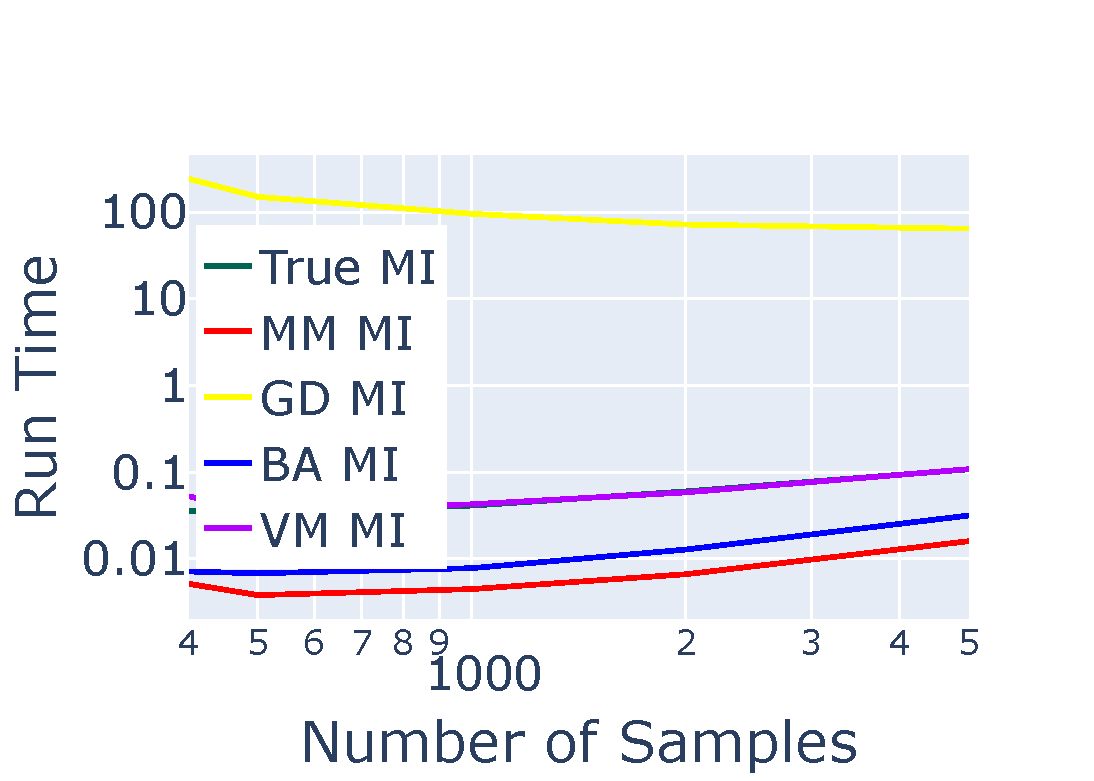
\includegraphics[width=.36\textwidth]{LargeGMMTime.pdf}
    }
    \hspace*{-6mm}\subfigure[GD Convergence]{
        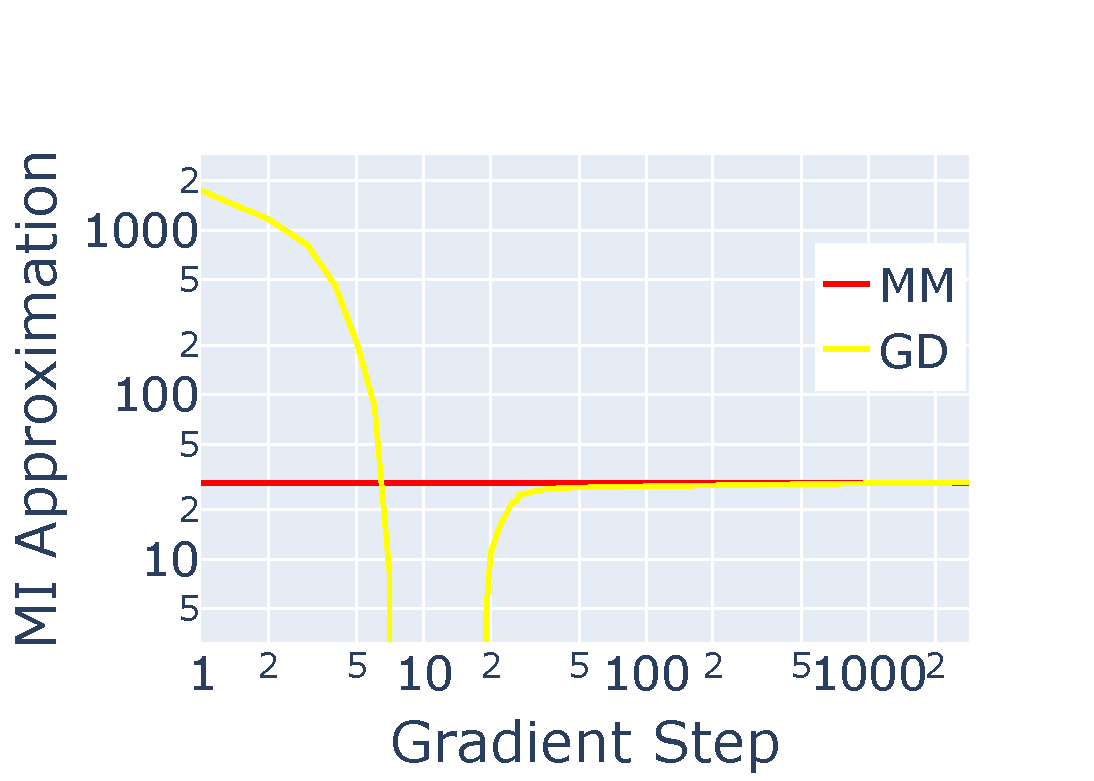
\includegraphics[width=.36\textwidth]{GMMGDStep.pdf}
    }    
    \hspace*{-6mm}\subfigure[MI Convergence]{
    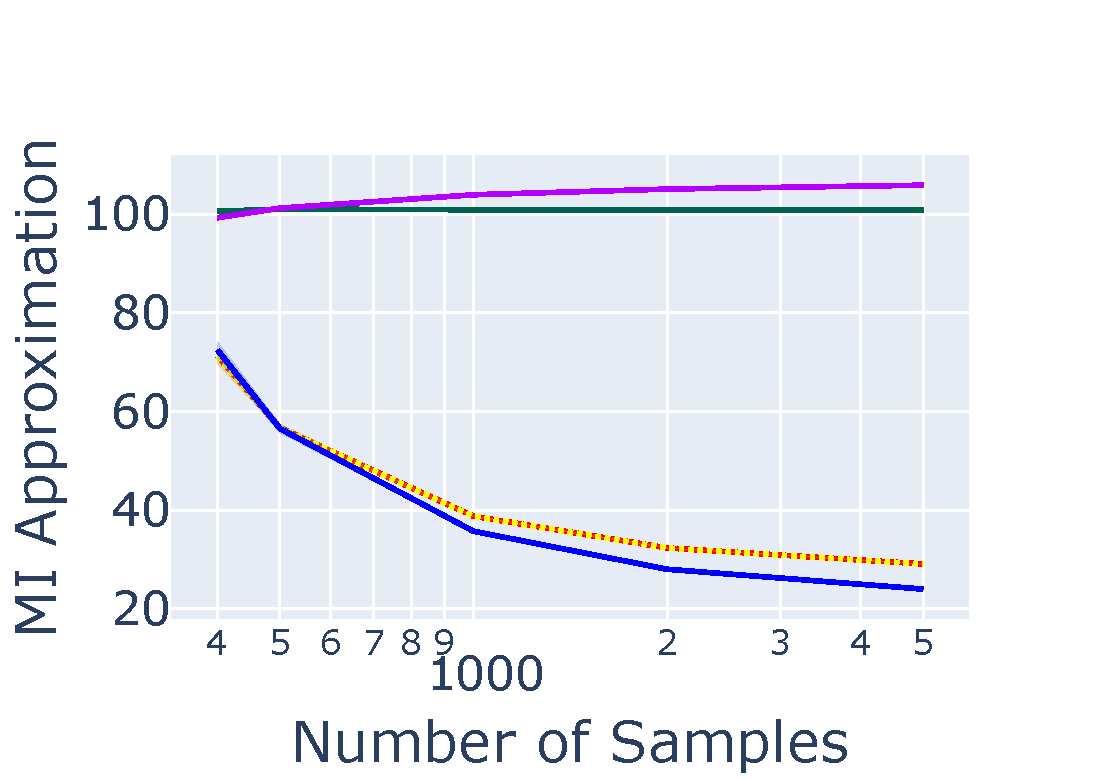
\includegraphics[width=.36\textwidth]{LargeGMMConverge.pdf}
    }
  \end{tabular}
    \caption{\small\textbf{High-dimensional Bimodal GMM.} Moment
      matching estimates have orders of magnitude lower computation as
      a function of sample size (a).  As per our theoretical analysis,
      our moment-matching solution to $\Iml$ achieves the same
      estimate while avoiding gradient iterations (b).  In this model
      we see that $\Imarg$ yields the most accurate estimates.  ``True
      MI'' is calculated via Monte Carlo estimation with exact
      evaluation of the model probabilities.}
    \label{fig:LargeGMMConvergence}
    \end{figure*}

%% sample convergence (right) for each method. We see that each
%% approximation satisfies the theoretical bounds discussed, with
%% $\Ipost$ as a lower bound, $\Imarg$ as an upper bound, and $\Iml$
%% lying inbetween. We can observe the computation times in this high
%% dimensional case. The true MI is more computationally intensive in
%% this scenario so we see that Moment Matching is slighly faster than
%% computing $\Imarg$ and $\Ipost$.

%% A synthetic model is constructed for explicit comparing of methods. In these 
%% experiments, a multivariate Gaussian Mixture Model with $K$ modes, latent 
%% variable dimension $D_x$, and observation variable dimension $D_y$ , is generated 
%% as the joint distribution. Samples can be directly drawn from the prior and 
%% then the posterior as $x_n\sim p(x)$ and $y_n\sim p(y|x=x_n)$. Since the true 
%% distributions are known, the true entropy can be numerically calculated using 
%% these samples. We will compare each of the methods to this numerical calculation.\\

%% The GMM we will consider will have high dimensions, with $K=2$, $D_x=100$ 
%% and $D_y = 200$. The purpose of this will be to emphasis the efficiency of 
%% calculating MM approximation over the Varaitional Marginal, Variational Posterior,
%% and especially over Gradient Descent. \\

%% Most importantly, moment matching is orders of magnitude faster than
%% computing the Gradient Descent approach for the exact same
%% approximation. To emphasis this result, consider the convergence of
%% gradient descent in Figure \ref{fig:LargeGMMConvergence}
%% (right). 

%% Using Moment Mathcing for $\Iml$, notice that we get similar quality approximations
%% to MI while saving drastic compution time. In a scenario with even higher 
%% dimensionality or a large domain of decisions, the computational speed up of Moment
%% Matching is drastic compared to $\Imarg$, $\Ipost$, and especially $\hat{I}_{NMC}$.


% \begin{figure*}[!htb]
%     \centering
%     \subfigure[MI Convergence]{
%     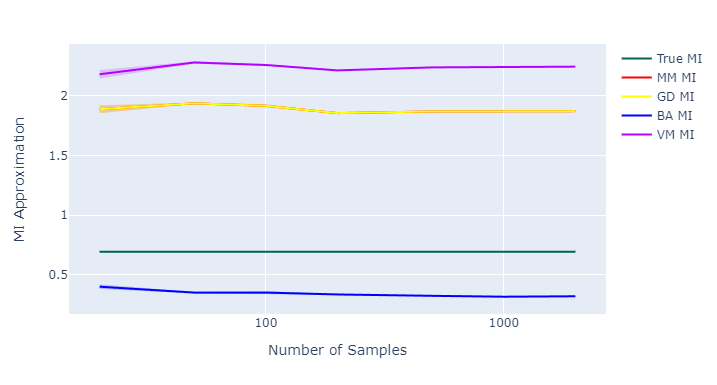
\includegraphics[width=.34\textwidth]{GMMMI.png}
%     }
%     \subfigure[Computation Time]{
%     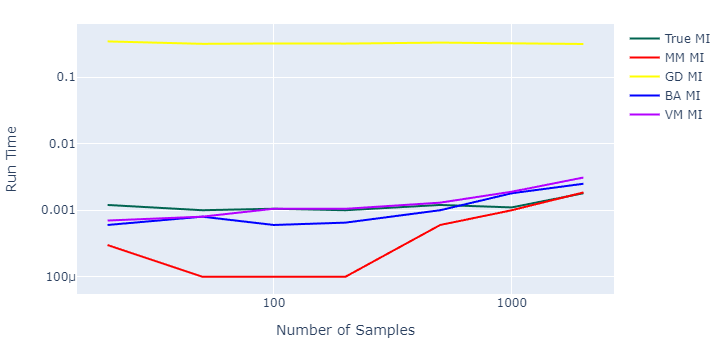
\includegraphics[width=.34\textwidth]{GMMTime.png}
%     }
%     \subfigure[Samples]{
%     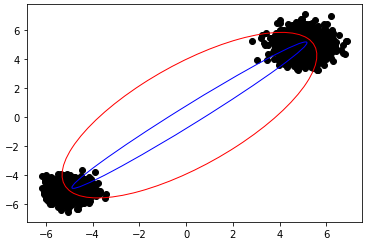
\includegraphics[width=.26\textwidth]{GMMSample.png}
%     }
%     \caption{\textbf{Gaussian Mixture Model Mutual Information Estimation} A Guassian Mixture model with 2 modes and Dimensions of Latent Variable, $X$, and Observation Variable $Y$, both being $1$. (a) The convergence of MI with respect to the number of samples drawn is plotted (b) The run time of each method is plotted for the number of samples. (c) The plotted samples drawn with an overlayed Moment Matched Gaussian Variational Approximation and an "Oracle" Gaussian approximation that matches the true Mutual Information. Variational Marginal is and upper bound, Variational Posterior is a lwoer bound, and MM/GD is a closer upper bound.}
%     \label{fig:GMMConvergence}
%     \end{figure*}
% Likewise, we can compute and "oracle" variational distribution which learns 
% it parameters by minimizing the absolute difference in the numerical Mutual 
% Information to the Implicit Likelihood approximation. This will be used to 
% qualitatively compare against the learned moment matching distribution.
% The first GMM we will consider will have $K=2$, $D_x=1$, and $D_y=1$. 
% Figure \ref{fig:GMMConvergence} show the convergence rate and time of each 
% methods. Now that our model is no longer linear gaussian, we see that the bound 
% of each methods holds as the bias introduced due to the plug in estimator is 
% negligible with respect to the varitional bounds. We again notice that each 
% method is significantly faster than that of the Gradient Descent.\\

% Figure \ref{fig:GMMConvergence} shows the sampled points along with the 
% Moment Match distribution and the Oracle distribution. We notice that both 
% share many similar quantities however the Oracle is a has larger variance 
% in on direction. This is responsible for lowering the Mutual Information to 
% match the True Mutual information by creating more uncertainty in the added 
% variance. This shows where the information is lost in Moment Matching for this 
% example.\\
